\lstinputlisting[language=bash,basicstyle=\small]{python_codes/fieldstone_79/keywords.ascii}

\begin{center}
Code at \url{https://github.com/cedrict/fieldstone/tree/master/python_codes/fieldstone_79}
\end{center}

\par\noindent\rule{\textwidth}{0.4pt}

{\sl This stone was developed in collaboration with Jort Jansen}. \index{contributors}{J. Jansen}

\par\noindent\rule{\textwidth}{0.4pt}

%%%%%%%%%%%%%%%%%%%%%%%%%%%%%%%%%%%%%%%%%%%%%%%%%%%%%%%%%%%%%%%%%%%%%%%%%%%%%%%%%%%%%%%%

Before reading what follows I urge you to go to Chapter~\ref{MMM-dgfem}. The derivations 
presented therein are long and complex, but absolutely necessary to make sense of the code.  
The code has been written for both bilinear ($Q_1$) quadrilateral elements and 
and linear ($P_1$) triangular elements. Meshes are then as follows:

\begin{center}
\includegraphics[width=10cm]{python_codes/fieldstone_79/images/grids2D_tris}\\
{\captionfont Example of a $4\times 3$ triangular mesh.}
\end{center}

\begin{center}
\includegraphics[width=10cm]{python_codes/fieldstone_79/images/grids2D_quads}\\
{\captionfont Example of a $4\times 3$ quadrilateral mesh.}
\end{center}

Contrarily to standard continuous finite elements nodes/vertices are not 
shared across elements so that the node layout is entirely based on the 
already built connectivity array {\tt icon}. Node coordinates are stored in 
{\tt xT} and {\tt yT}.

Six ascii output files are opened at the beginning of the code, and in these 
various statistics will be written out. These are 
{\sl T\_stats.ascii}, {\sl qx\_stats.ascii}, {\sl qy\_stats.ascii},
{\sl residual\_T\_stats.ascii}, {\sl residual\_qx\_stats.ascii}, and {\sl residual\_qy\_stats.ascii}.

Then a large number of arrays is declared. Then contain information that is needed 
when building the matrices and vectors later on and it is convenient to store this information
beforehand. They all start with {\tt edge} and record the normal to the edge, its center coordinates, 
its length, whether it is on the domain boundary, etc ... Because this is an educative code 
with a simple mesh topology we can directly ascribe the normals to each side. If a mesher, like 
Triangle \cite{shew14}, was used then we would need to compute the normals to each side by means
of simple geometrical considerations.

We continue to build the necessary arrays pertaining to neighbours. 
We build the {\tt edgeX\_neighb[iel]} arrays which contain the identity of the element 
on the other size of edge X of element iel.
For instance, looking at the example above of a triangular mesh, we have
\begin{lstlisting}
edge1_neighb[0]=-1
edge2_neighb[0]=1
edge3_neighb[0]=-1
...
edge1_neighb[10]=3
edge2_neighb[10]=11
edge3_neighb[10]=9
\end{lstlisting}
where the -1 value indicates that there is no element neighbour.

We then build the arrays {\tt edgeX\_neighbedge[iel]} (where X stand for 1, 2, 3, 
or 4) which stores the identity/number of the edge on the element across the common face
(if there is a neighbour).
For instance:
\begin{lstlisting}
edge1_neighbedge[10]=2
edge2_neighbedge[10]=3
edge3_neighbedge[10]=1
\end{lstlisting}


\begin{center}
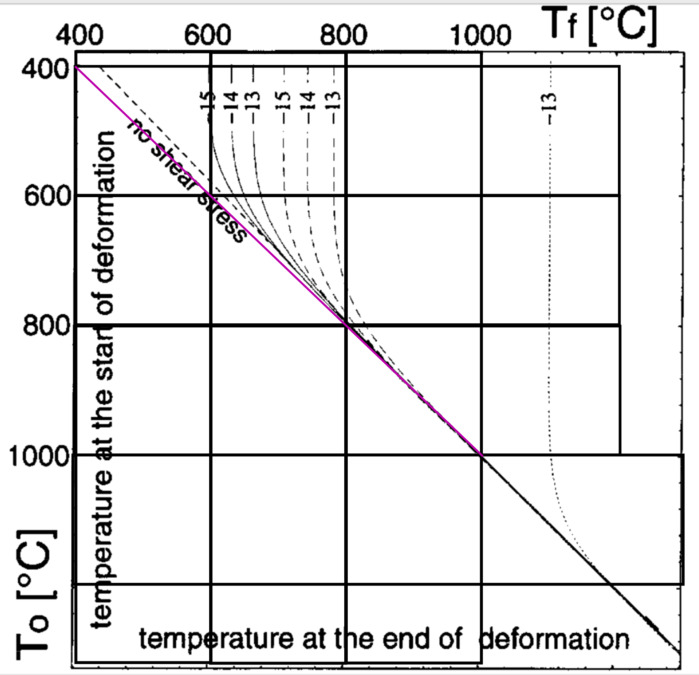
\includegraphics[width=10cm]{python_codes/fieldstone_79/images/drawing}\\
{\captionfont When two triangles are neighbours (here along edge 1
of grey triangle) three configurations can occur.}
\end{center}

%............................
\paragraph{Iterative process}
Although we are solving the steady-state diffusion equation, we still need to carry out 
iterations (this is a consequence of the DG formulation itself and it is not the 
case for 'regular' finite elements).
These iterations are implemented as follows:
\begin{lstlisting}
for iter in range(0,niter):
\end{lstlisting}
where {\tt niter} is set to 100. Vector residuals are computed for $T$, $q_x$ and $q_y$. When the
infinite-norm of all three is below the tolerance {\tt tol} then the system is considered 
converged and iterations are stopped.   
For each iteration the code prints a number of helpful statistics in the terminal:
\begin{scriptsize}
\begin{verbatim}
iter=   0 : T,qx,qy (m/M)= 6.944e-03 2.053e+00 | -1.067e+01 2.054e+01 | -1.067e+01 2.054e+01 | max(resT)= 5.700e-01 (tol= 1.0e-09)
iter=   1 : T,qx,qy (m/M)= 9.982e-04 2.053e+00 | -3.991e+00 8.163e+00 | -3.991e+00 8.163e+00 | max(resT)= 7.515e-01 (tol= 1.0e-09)
iter=   2 : T,qx,qy (m/M)= 9.982e-04 2.702e+00 | -2.278e+00 3.863e+00 | -2.278e+00 3.863e+00 | max(resT)= 5.316e-01 (tol= 1.0e-09)
...
iter=  41 : T,qx,qy (m/M)= 3.473e-13 2.000e+00 | 1.000e+00 1.000e+00 | 1.000e+00 1.000e+00 | max(resT)= 1.537e-09 (tol= 1.0e-09)
iter=  42 : T,qx,qy (m/M)= 3.473e-13 2.000e+00 | 1.000e+00 1.000e+00 | 1.000e+00 1.000e+00 | max(resT)= 9.357e-10 (tol= 1.0e-09)
\end{verbatim}
\end{scriptsize}

Each iteration consists in a sweep through elements and we implement a forward-backward scheme:
even-numbered iterations got from 0 to nel-1, while odd-numbered ones go from nel-1 down to 0:
\begin{lstlisting}
if iter%2==0:
   start=0
   end=nel
   step=1
else:
   start=nel-1
   end=-1
   step=-1
\end{lstlisting}





\newpage

Explore/implement

source term
randomised nodes so no right angles




%------------------------------------------------
\subsubsection*{Experiment \#1 - testing signs} 

We define the simple temperature field 
\[
T(x,y)=x+y
\]
over a unit square domain, so that (taking $k=1$) we have
\[
q_x(x,y)=-1
\qquad
q_y(x,y)=-1
\]
I prescribe this temperature on all four sides of the domain. 

\begin{center}
\includegraphics[width=5cm]{python_codes/fieldstone_79/results/exp1/temp}
\includegraphics[width=5cm]{python_codes/fieldstone_79/results/exp1/temp2}
\end{center}


VERIFY: minus sign problem for heat fluxes ?


%------------------------------
\subsubsection*{Experiment \#2 - testing symmetry} 

On all four sides of the domain the temperature $T(x,y)=x(L_x-x)+y(L_y-y)$
is prescribed. There is no analytical solution to this problem (?) but 
it allows us to test that the solution is symmetric as expected.

\begin{center}
\includegraphics[width=5cm]{python_codes/fieldstone_79/results/exp2/temp}
\includegraphics[width=5cm]{python_codes/fieldstone_79/results/exp2/temp2}
\end{center}




